\documentclass[14pt]{extbook}
\usepackage{multicol, enumerate, enumitem, hyperref, color, soul, setspace, parskip, fancyhdr} %General Packages
\usepackage{amssymb, amsthm, amsmath, latexsym, units, mathtools} %Math Packages
\everymath{\displaystyle} %All math in Display Style
% Packages with additional options
\usepackage[headsep=0.5cm,headheight=12pt, left=1 in,right= 1 in,top= 1 in,bottom= 1 in]{geometry}
\usepackage[usenames,dvipsnames]{xcolor}
\usepackage{dashrule}  % Package to use the command below to create lines between items
\newcommand{\litem}[1]{\item#1\hspace*{-1cm}\rule{\textwidth}{0.4pt}}
\pagestyle{fancy}
\lhead{Module2}
\chead{}
\rhead{Version B}
\lfoot{3163-1865}
\cfoot{}
\rfoot{test}
\begin{document}

\begin{enumerate}
\litem{
Write the equation of the line in the graph below in Standard form $Ax+By=C$. Then, choose the intervals that contain $A, B, \text{ and } C$.
\begin{center}
    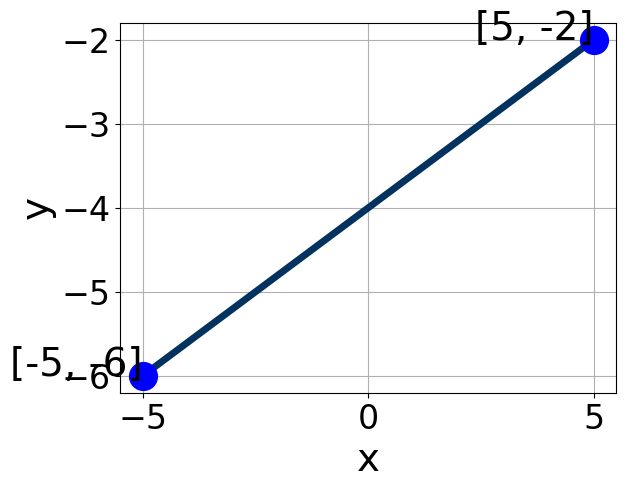
\includegraphics[width=0.5\textwidth]{../Figures/linearGraphToStandardB.png}
\end{center}
\begin{enumerate}[label=\Alph*.]
\item \( A \in [4, 6], \hspace{3mm} B \in [1.92, 2.48], \text{ and } \hspace{3mm} C \in [-12.4, -8.9] \)
\item \( A \in [1.5, 4.5], \hspace{3mm} B \in [0.54, 1.54], \text{ and } \hspace{3mm} C \in [-7.4, -3.8] \)
\item \( A \in [4, 6], \hspace{3mm} B \in [-2.61, -1.41], \text{ and } \hspace{3mm} C \in [7.4, 12.2] \)
\item \( A \in [1.5, 4.5], \hspace{3mm} B \in [-1.2, -0.68], \text{ and } \hspace{3mm} C \in [2.6, 7.8] \)
\item \( A \in [-6, 1], \hspace{3mm} B \in [-2.61, -1.41], \text{ and } \hspace{3mm} C \in [7.4, 12.2] \)

\end{enumerate} }
\litem{
First, find the equation of the line containing the two points below. Then, write the equation as $ y=mx+b $ and choose the intervals that contain $m$ and $b$.\[ (-11, 3) \text{ and } (-5, -10) \]\begin{enumerate}[label=\Alph*.]
\item \( m \in [1.4, 3.4] \hspace*{3mm} b \in [-0.17, 1.83] \)
\item \( m \in [-2.4, 0.3] \hspace*{3mm} b \in [-22.83, -14.83] \)
\item \( m \in [-2.4, 0.3] \hspace*{3mm} b \in [11, 18] \)
\item \( m \in [-2.4, 0.3] \hspace*{3mm} b \in [-9, -4] \)
\item \( m \in [-2.4, 0.3] \hspace*{3mm} b \in [20.83, 25.83] \)

\end{enumerate} }
\litem{
Solve the equation below. Then, choose the interval that contains the solution.\[ -18(13x -2) = -19(3x + 6) \]\begin{enumerate}[label=\Alph*.]
\item \( x \in [0.39, 0.62] \)
\item \( x \in [-0.46, -0.28] \)
\item \( x \in [0.81, 1] \)
\item \( x \in [-0.36, -0.24] \)
\item \( \text{There are no real solutions.} \)

\end{enumerate} }
\litem{
Find the equation of the line described below. Write the linear equation as $ y=mx+b $ and choose the intervals that contain $m$ and $b$.\[ \text{Perpendicular to } 5 x + 3 y = 12 \text{ and passing through the point } (10, -7). \]\begin{enumerate}[label=\Alph*.]
\item \( m \in [-0.13, 1.47] \hspace*{3mm} b \in [-22, -15] \)
\item \( m \in [-0.13, 1.47] \hspace*{3mm} b \in [-13, -9] \)
\item \( m \in [-1.48, -0.09] \hspace*{3mm} b \in [-3, 0] \)
\item \( m \in [-0.13, 1.47] \hspace*{3mm} b \in [12, 14] \)
\item \( m \in [1.61, 2.34] \hspace*{3mm} b \in [-13, -9] \)

\end{enumerate} }
\litem{
Write the equation of the line in the graph below in Standard form $Ax+By=C$. Then, choose the intervals that contain $A, B, \text{ and } C$.
\begin{center}
    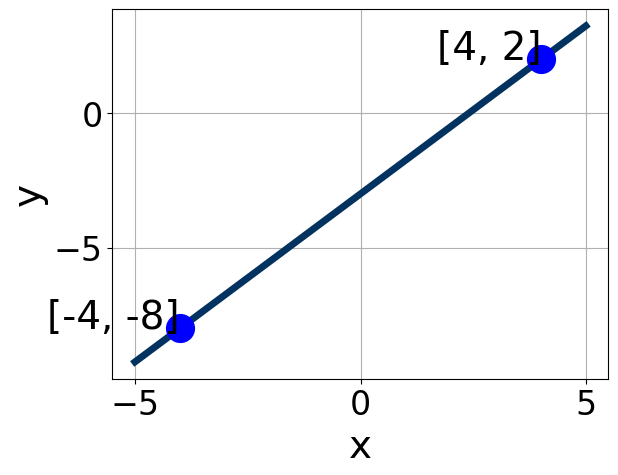
\includegraphics[width=0.5\textwidth]{../Figures/linearGraphToStandardCopyB.png}
\end{center}
\begin{enumerate}[label=\Alph*.]
\item \( A \in [-2.1, -0.7], \hspace{3mm} B \in [4.9, 7.1], \text{ and } \hspace{3mm} C \in [18, 25] \)
\item \( A \in [-1.7, -0.2], \hspace{3mm} B \in [-2.5, 0.8], \text{ and } \hspace{3mm} C \in [-6, 2] \)
\item \( A \in [1.3, 3.7], \hspace{3mm} B \in [4.9, 7.1], \text{ and } \hspace{3mm} C \in [18, 25] \)
\item \( A \in [1.3, 3.7], \hspace{3mm} B \in [-7.6, -3.4], \text{ and } \hspace{3mm} C \in [-21, -16] \)
\item \( A \in [-1.7, -0.2], \hspace{3mm} B \in [-0.5, 2.9], \text{ and } \hspace{3mm} C \in [0, 5] \)

\end{enumerate} }
\litem{
Find the equation of the line described below. Write the linear equation as $ y=mx+b $ and choose the intervals that contain $m$ and $b$.\[ \text{Perpendicular to } 4 x + 9 y = 13 \text{ and passing through the point } (6, -7). \]\begin{enumerate}[label=\Alph*.]
\item \( m \in [0.6, 3.7] \hspace*{3mm} b \in [-20.5, -17.5] \)
\item \( m \in [0.6, 3.7] \hspace*{3mm} b \in [14.5, 25.5] \)
\item \( m \in [0.6, 3.7] \hspace*{3mm} b \in [-15, -9] \)
\item \( m \in [-2.2, 1.4] \hspace*{3mm} b \in [-20.5, -17.5] \)
\item \( m \in [-2.3, -2.1] \hspace*{3mm} b \in [6.5, 8.5] \)

\end{enumerate} }
\litem{
First, find the equation of the line containing the two points below. Then, write the equation as $ y=mx+b $ and choose the intervals that contain $m$ and $b$.\[ (-7, -7) \text{ and } (4, -10) \]\begin{enumerate}[label=\Alph*.]
\item \( m \in [-0.88, -0.2] \hspace*{3mm} b \in [-16.8, -11.2] \)
\item \( m \in [0.18, 0.57] \hspace*{3mm} b \in [-12.3, -9.3] \)
\item \( m \in [-0.88, -0.2] \hspace*{3mm} b \in [-3.5, 0.8] \)
\item \( m \in [-0.88, -0.2] \hspace*{3mm} b \in [-10.7, -6.9] \)
\item \( m \in [-0.88, -0.2] \hspace*{3mm} b \in [6.8, 10.1] \)

\end{enumerate} }
\litem{
Solve the linear equation below. Then, choose the interval that contains the solution.\[ \frac{3x -5}{4} - \frac{5x + 5}{7} = \frac{4x + 9}{3} \]\begin{enumerate}[label=\Alph*.]
\item \( x \in [-4.24, -3.2] \)
\item \( x \in [-14.7, -14.31] \)
\item \( x \in [-3.18, -2.02] \)
\item \( x \in [-1.99, -0.58] \)
\item \( \text{There are no real solutions.} \)

\end{enumerate} }
\litem{
Solve the linear equation below. Then, choose the interval that contains the solution.\[ \frac{3x -6}{5} - \frac{-4x + 5}{6} = \frac{5x + 9}{4} \]\begin{enumerate}[label=\Alph*.]
\item \( x \in [1.14, 4.14] \)
\item \( x \in [1200, 1202] \)
\item \( x \in [253, 258] \)
\item \( x \in [157, 159] \)
\item \( \text{There are no real solutions.} \)

\end{enumerate} }
\litem{
Solve the equation below. Then, choose the interval that contains the solution.\[ -3(-14x + 10) = -12(4x -15) \]\begin{enumerate}[label=\Alph*.]
\item \( x \in [-3, -1.6] \)
\item \( x \in [0.7, 2.1] \)
\item \( x \in [2.2, 2.7] \)
\item \( x \in [24.1, 25.3] \)
\item \( \text{There are no real solutions.} \)

\end{enumerate} }
\end{enumerate}

\end{document}